\section{Self-confidence Factorization and Calculation} \label{sec:self-confidence}
    \begin{figure}[tbp]
        \centering
        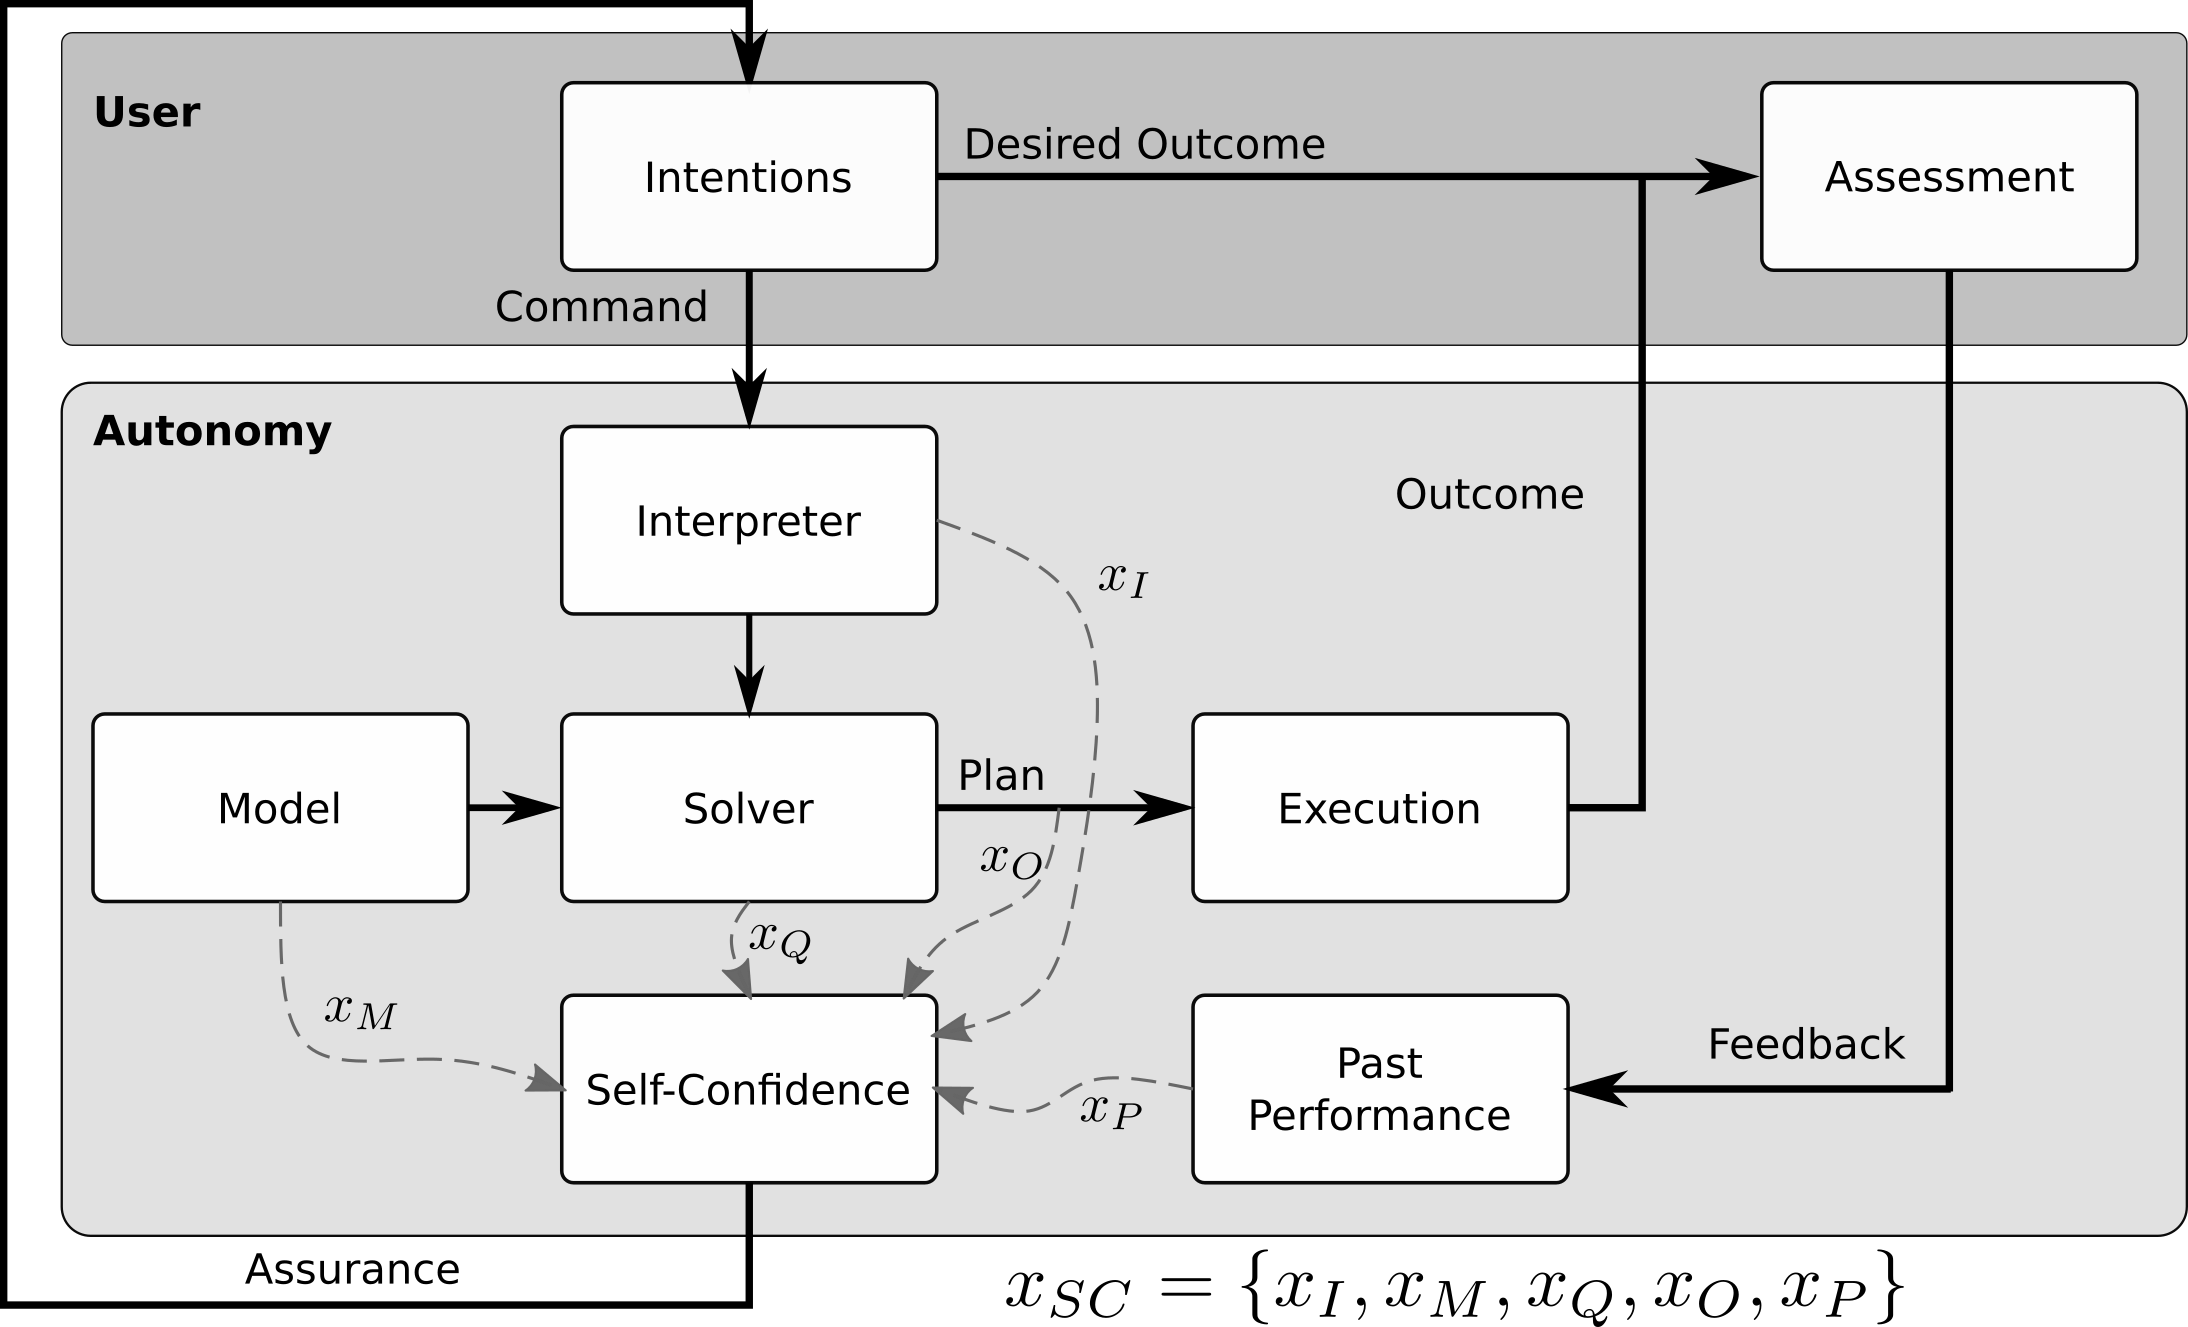
\includegraphics[width=0.80\linewidth]{Figures/FaMSeC.png}
        \caption{Factorized Machine Self-Confidence (\famsec)}
        \label{fig:famsec}
        \vspace{-0.5cm}
    \end{figure}
    
    This work seeks to develop algorithmic strategies for assessing and communicating machine self-confidence. Of particular interest are model-based techniques that endow an APS with a process-driven scoring of how it arrives at decisions, and what factors influence the quality of its reasoning, in order to quantitatively assess its own competency boundaries. As such, it is important to formally establish both: (i) a set of principles, definitions, and relations that govern the `arithmetic of machine self-confidence' as a function of task, environment, system realization, and context, and (ii) variables, representations and operations for producing meaningful self-confidence assessments. 
    
    We initially address these issues for APS that are primarily defined by capabilities for dynamic decision-making and planning under uncertainty. This approach provides a pathway to developing firm initial mathematical and computational bases for addressing (i) and (ii) via the rich set of analytical and computational features inherent to the MDP model family. %Insights developed along these lines can provide the basis of future work for formulating self-confidence computation strategies, other important planning model families, and APS capabilities that are formally related to decision making under uncertainty, such as dynamic learning and partially observable planning with sensing and perception. 
    After reviewing a computational framework for self-confidence assessment that relies on assessing individual factors involved with solving MDP-based planning and decision-making problems, we consider how one of these factors (related to the quality of a given MDP policy solver) can actually be computed, building on insights derived from calculation and analysis of another factor (related to intrinsic task difficulty) examined in other work. 
    
    \subsection{The \famsec{} Framework }
    The approach presented here adopts and builds on the \emph{Factorized Machine Self-Confidence (\famsec)} framework developed in ref. \cite{Aitken2016-cv, Aitken2016-fb}. The key idea behind \famsec{} is to represent and compute self-confidence as a traceable multi-factor function, which combines shorthand assessments of where and when operations and approximations inherent to model-based autonomous decision-making are expected to break down. As with the self-confidence reporting strategy developed in \cite{Hutchins2015-if}, this captures metrics than an expert designer would use to assess the correctness and quality of an autonomous decision-making system, accounting for variations in task, environment, system implementation, and context. However, unlike \cite{Hutchins2015-if}, \famsec{} allows an APS to automatically generate its own holistic assessments of self-confidence, i.e. without the need for a human designer/expert to specify a priori how self-confident a system ought to be given such variations %%(which can be cumbersome, if not impossible, to fully account for in practical applications). 
    
    Figure \ref{fig:famsec} illustrates \famsec's notional overall self-confidence scoring mechanism. This uses a set of \emph{self-confidence factors} (dashed lines) that are derived from core algorithmic decision-making components (white boxes in the `Autonomy' block). The total self-confidence score can be mapped onto an arbitrary scale, e.g. -1 to +1 for the sake of discussion, where -1 gives a shorthand indication of `complete lack of confidence' (i.e. some aspect of task, environment, or context falls completely outside the system's competency boundaries), and +1 indicates `complete confidence' (i.e. all aspects of task, environment, and mission context are well within system's competency boundaries). As will be shown later, the scales for each factor need not all be the same and can carry slightly different qualitative interpretations, as long as a clear sense of `confidence direction' (i.e. degree of self-trust) can be established for each. 
    Ref. \cite{Aitken2016-cv} considers five general factors that contribute to a `total self-confidence score', which notionally maps the multivariate the combined set of individual factors into an overall confidence report:
    
    
\begin{enumerate}
    \item \xI---\textit{\textbf{interpretation of user intent and task}}: To what extent were the user's intentions properly understood and translated by the autonomous system into context-appropriate mission specifications and tasks?
    
    \item \xM---\textit{\textbf{model and data validity}}: Are the agent's learned and/or assumed models, and associated training data used for decision-making good enough proxies for the real world?
    
    \item \xQ---\textit{\textbf{solver quality}}: Are the approximations and learning-based adaptations used by the system for solving decision-making problems appropriate for the given mission and model? 
    
    \item \xO---\textit{\textbf{expected outcome assessment}}: Do the sets of possible events, rewards, costs, utilities, etc. for a particular decision lead to desirable outcomes? 
    
    \item \xP---\textit{\textbf{past history and experiences}}: What can be gleaned from the system's own experience and other available historical information for past problem instances?  
\end{enumerate}

Since the overall self-confidence mapping is heavily dependent on application, context, and desired levels/types of user-autonomy interaction, this work assumes for simplicity that the overall mapping consists of a direct report of some fixed subset of the component factors, i.e. \xSC. 
Furthermore, the five factors considered here are neither exclusive nor exhaustive. For example, the factors developed by \cite{Aitken2016-cv, Aitken2016-fb} are primarily aimed at self-assessment \emph{prior} to the execution of a particular task, whereas it is conceivable that other self-confidence factors could be included to account for in situ and post hoc self-assessments. For simplicity, attention is restricted to the a priori task self-assessment case. %%\nisar{where is traceability mentioned?  notional ability for user to `drill down'?}
